\documentclass{article}[18pt]
\usepackage{../../../../../format}
\lhead{ADS - Andrei}
\usepackage{tikz}

\lstset{language=Python,
	basicstyle=\ttfamily,
	keywordstyle=\bfseries,
	showstringspaces=false,
	morekeywords={if, else, then, print, end, for, do, while, parallel},
	tabsize=4,
	mathescape=true
}

\usepackage[trim]{tokenizer} 

\makeatletter

\newcounter{sncolumncounter}
\newcounter{snrowcounter}

\def \nodelabel#1{%
	\setcounter{snrowcounter}{1}
	\foreach \i in {#1}{%
		\draw (\value{sncolumncounter},\value{snrowcounter}) node[anchor=south]{\i};
		\addtocounter{snrowcounter}{1}
	}
	\addtocounter{sncolumncounter}{1}
}

\def \nodeconnection#1{%
	\foreach \i in {#1}{%
		\GetTokens{nodesrc}{nodedest}{\i}
		\draw (\value{sncolumncounter},\nodesrc) node[circle,fill=black]{}--(\value{sncolumncounter},\nodedest) node[circle,fill=black]{};
	}
	\addtocounter{sncolumncounter}{1}
}

\newenvironment{sortingnetwork}[3]
{
	\setcounter{sncolumncounter}{0}
	\def \sn@fullsize{15}
	\begin{tikzpicture}[scale=#3*\sn@fullsize/#2]
	\foreach \i in {1, ..., #1}
	{
		\draw (0,\i)--(#2-1,\i);
	}
}
{
	\end{tikzpicture}
}
\makeatother

% Sequence
\newcommand{\seq}[3]{#1_{#2}\ldots#1_{#3}}

% Make paragraphs formatted like sections
\setcounter{secnumdepth}{4}

\begin{document}
\begin{center}
\underline{\huge Sorting Part 3}
\end{center}
\section{Networks}
\subsection{Comparator}
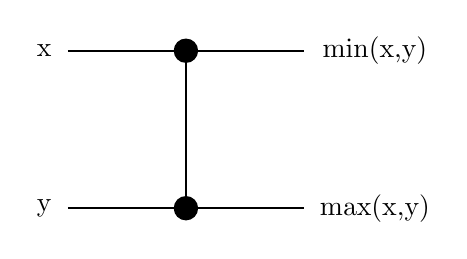
\begin{tikzpicture}
\draw[black, thick] (0,0) -- (3,0) node[pos=-0.1]{x} node[pos=1.3]{min(x,y)};
\filldraw[black,thick] (1.5,0) circle (4pt);
\draw[black, thick] (0,-2) -- (3,-2) node[pos=-0.1]{y} node[pos=1.3]{max(x,y)};
\filldraw[black,thick] (1.5,-2) circle (4pt);
\draw[black,thick] (1.5,0)--(1.5,-2);
\end{tikzpicture}\\
This works in $\mathcal{O}(1)$ time\\
\begin{sortingnetwork}{4}{9}{0.5}
	\nodelabel{6,2,5,9}
	\nodeconnection{{1,2},{3,4}}
	\nodelabel{6,2,9,5}
	\nodeconnection{{2,4}}
	\nodelabel{6,5,9,2}
	\nodeconnection{{1,3}}
	\nodelabel{9,5,6,2}
	\nodeconnection{{2,3}}
	\nodelabel{9,6,5,2}
\end{sortingnetwork}
\\
Wires go straight, left to right\\
Each comparator has inputs/outputs on some pairs of wires\\
Data marches left to right, in goose step (synchronised)\\
\\
The depth is the longest chain of comparators that could be encountered, so the above example has depth of 3
\subsection{Claim}
This comparison network will sort any set of 4 input values
\subsection{Proof}
\begin{itemize}
	\item after leftmost comparators, min is on either wire 1 or 3, max is on either 2 or 4
	\item after next two comparators, min is on wire 1, max on 4
	\item last comparator gets correct values onto 2 and 3
\end{itemize}
\subsection{Selection sorter}
\begin{center}
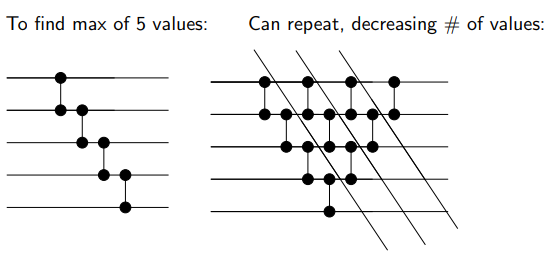
\includegraphics[scale=0.7]{selection}
\end{center}
Depth: $D ( n ) = D ( n - 1 ) + 2 , D ( 2 ) = 1 \Rightarrow D ( n ) = 2 n - 3 = \Theta ( n )$\\
If view depth as "time" parallelism gets us faster method than any sequential comparison based sort
\subsection{Can we do better}
We can do better than $\Theta(n)$, the AKS network has depth $\mathcal{O}(\log n)$, with the caveats:
\begin{itemize}
\item Huge constant
\item Really hard to construct
\item Highly impractical - of theoretical interest only 
\end{itemize}
\subsection{Simplification}
\begin{itemize}
	\item Consider the line (1D array) of length n
	\item Each node 1,\ldots,n stores one of the items to be sorted
	\item in even steps even-numbered nodes i compare/exchange with their neighbour i+1
	\item in odd steps odd-numbered nodes i compare/exchange with their neighbour i+1
	\item called \textbf{odd-even transposition sort} (OETS)
\end{itemize}
For example:
\begin{center}
	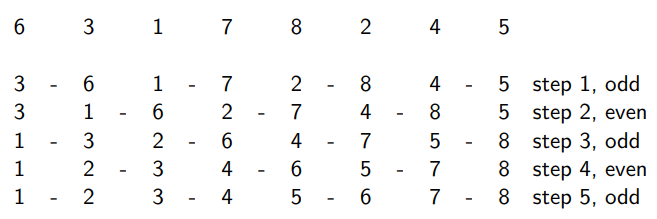
\includegraphics[scale=0.7]{network}
\end{center}
This is very similar to \textbf{bubble sort}\\
\\
The questions are now:
\begin{itemize}
	\item does it always work? yes
	\item how long does it take? no more than n steps
\end{itemize}
It can be viewed as a sorting network of depth n:
\begin{center}
	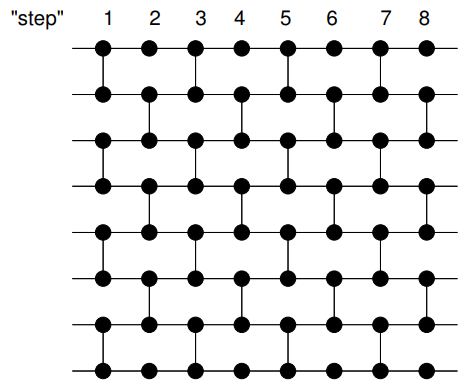
\includegraphics[scale=0.7]{network1}
\end{center}
We will prove this using the 0/1 principle and induction\\
\\
\textbf{Lemma (0-1 principle)}\\
Let CE be an \textbf{oblivious compare-exchange algorithm} or network. CE correctly sort all sequences of integer numbers iff CE correctly sorts all 0-1 sequences\\
\\
\\ Oblivious - does the same steps no matter what the values of the input is\\
\textbf{Lemma(OETS)}\\
An OETS network of depth n sorts any input of length n\\
\\
\textbf{Base: $n\leqslant 2$} clear (comparators work by definition)\\
\textbf{Step $n-1\rightarrow n$} Let N be OETS network for n elements and let $a=(a_0,...,a_{n-1})$ be 0/1 sequence\\
\\
\textbf{Case 1} if $a_{n-1}$ (bottom row) then:
\begin{itemize}
	\item bottom row of comparators obsolete
	\item we've got OETS network for n-1 elements plus superfluous row and column
	\item by hypothesis $(a_0,...,a_{n-2})$ get sorted
	\item $a_{n-1}$ already in proper position so we're done
\end{itemize}
\textbf{Case 2} if $a_{n-1}=0$ then
\begin{itemize}
	\item Any comparator seeing this 0 performs swap (if other element is also 0 then jump horses); might as well replace them with fixed crossing lines
	\begin{center}
		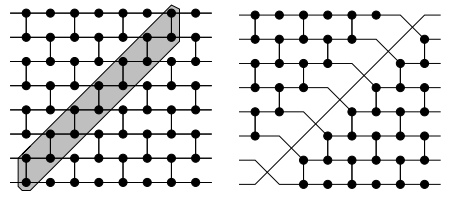
\includegraphics[scale=0.7]{networkProof}
	\end{center}
	\item What remains is OETS network for input size n-1 so we're done
\end{itemize}
\subsection{Proving the 0-1 Principle}
Assume you have an input
$<a_1,a_2,...,a_n>\xrightarrow[]{C}<b_1,b_2,...,b_n>$\\
You have a monotonic function $f:\mathbb{Z}\rightarrow\mathbb{Z}$\\
Where monotone is for every $x\leqslant y$ $\Rightarrow f(x)\leqslant f(y)$\\
Apply the monotonic function to a comparator\\
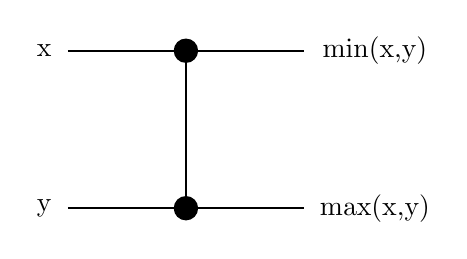
\begin{tikzpicture}
\draw[black, thick] (0,0) -- (3,0) node[pos=-0.1]{x} node[pos=1.3]{min(x,y)};
\filldraw[black,thick] (1.5,0) circle (4pt);
\draw[black, thick] (0,-2) -- (3,-2) node[pos=-0.1]{y} node[pos=1.3]{max(x,y)};
\filldraw[black,thick] (1.5,-2) circle (4pt);
\draw[black,thick] (1.5,0)--(1.5,-2);
\end{tikzpicture}\\
This would create\\
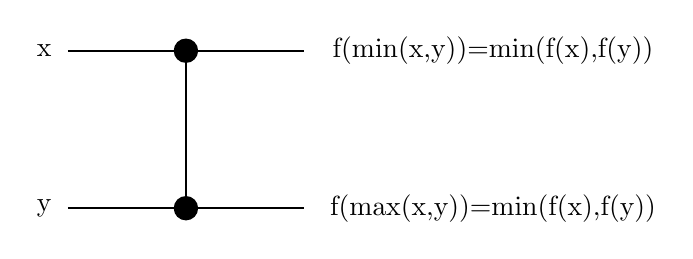
\begin{tikzpicture}
\draw[black, thick] (0,0) -- (3,0) node[pos=-0.1]{x} node[pos=1.8]{f(min(x,y))=min(f(x),f(y))};
\filldraw[black,thick] (1.5,0) circle (4pt);
\draw[black, thick] (0,-2) -- (3,-2) node[pos=-0.1]{y} node[pos=1.8]{f(max(x,y))=min(f(x),f(y))};
\filldraw[black,thick] (1.5,-2) circle (4pt);
\draw[black,thick] (1.5,0)--(1.5,-2);
\end{tikzpicture}\\
As this is true for a comparator, it will be true for any network of comparators\\
\\
Applying this to the sequence:\\
$<(f(a_1),f(a_2),...,f(a_n))>$$\xrightarrow{C}$$<f(b_1),f(b_2),...,f(b_n)>$\\
The winning elements of the first sequence($<a_1,a_2,...,a_n>\xrightarrow[]{C}<b_1,b_2,...,b_n>$) will be the same as the winning elements of this sequence\\
\\
Assume you have some input $a_1,a_2,...,a_i,...,a_j,...$ where $a_i>a_j$ and their order is maintained after going through the function, then the function is wrong.\\
\\
$$f(x)=\{ 0 \  if \  x<a_i \quad 1 \  if \  x\geqslant \  a_i\}$$
Out of this, you get a sequence of 0s and 1s sorted incorrectly.\\
\\
Want to prove C sorts 0-1 input $\Rightarrow$ sorts any input\\
\\
Proved it sorts some input incorrectly $\Rightarrow$ sorts some 0-1 input incorrectly (contrapositive proof)\\
\\
This is because in logic:
$$A\Rightarrow B \equiv \lnot B\Rightarrow\lnot A$$




\subsection{Bitonic sequences}
\textbf{Formal definition:} A sequence $(a_0,...,a_{n-1})$ is called \textbf{bitonic} if
\begin{enumerate}
	\item There is an index j, $0\leqslant j< n$ such that $(a_0,\ldots,a_j)$ is monotonically increasing , and $(a_j,\ldots ,a_{n-1})$ is monotonically decreasing
	\item if (1) is not fulfilled, then there is an index i, $0\leqslant i <n$ such that $(a_i,...,a_{n-1},a_0,...,a_{i-1})$ does fulfill (1). i.e. you can just loop the numbers round to the front (see example below)
\end{enumerate}
Examples:
\begin{itemize}
	\item (0,2,3,5,6,7,3,1) is bitonic by (1), j=5
	\item (6,7,5,3,0,1,4,5) is bitonic by (2), i=4, j=5, after shift: (0,1,4,5,6,7,5,3)
	\item An example of a non bitonic sequence is 1,3,2,4
\end{itemize}
All bitonic sequences of 0s and 1s are of the form:
\begin{itemize}
	\item $0^i1^j0^k$
	\item $1^i0^j1^k$
\end{itemize}
\subsubsection{"Shapes" of bitonic sequences}
\begin{center}
	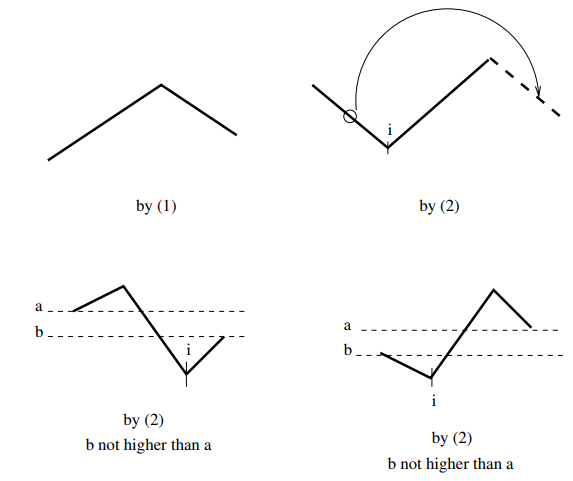
\includegraphics[scale=0.7]{shapes}
\end{center}
\subsubsection{Properties of bitonic sequences}
\begin{itemize}
	\item Property "bitonic" is closed under cyclic shift (remains bitonic under any cyclic shift)
	\item Every sub-sequence of a bitonic sequence is bitonic itself 
	\item If
$$A=(a_0,...,a_i)$$
monotonically increasing and
$$B=(b_{i+1},...,b_{n-1})$$
is monotonically decreasing, then
$$AB=(a_0,...,a_i,b_{i+1},b_{n-1})$$
is bitonic
\end{itemize}
\subsubsection{Bitonic sorting network}
\textbf{Step 1:} construct a "bitonic sorter"; it sorts any bitonic sequence\\
\\
For 0-1 sequences- which we can focus on - bitonic sequences have the form
$$0^i1^j0^k \quad \text{or} \quad 1^i0^j1^k$$
\\
\paragraph{Step 0: Half cleaner}
\begin{center}
	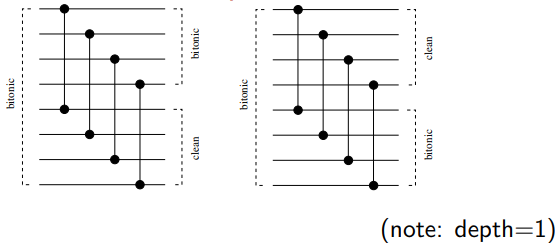
\includegraphics[scale=0.9]{half_cleaner}
\end{center}
If clean in lower part: all 1s\\
If clean in upper part: all 0s\\
\\
\textbf{Lemma}:\\
If the imput to a half-cleaner is a bitonic 0-1 sequence, then for output:
\begin{itemize}
	\item Both top and bottom half are bitonic
	\item every element in top half is $\leqslant$ any element in bottom half
	\item at least one of the halves is clean - all 0's or all 1's
\end{itemize}
\textbf{Proof:}\\
Sorter is comparing nth element in 1st half with nth element in 2nd half repeatedly for all elements\\

\paragraph{Step 1: Bitonic Sorter}
\begin{center}
	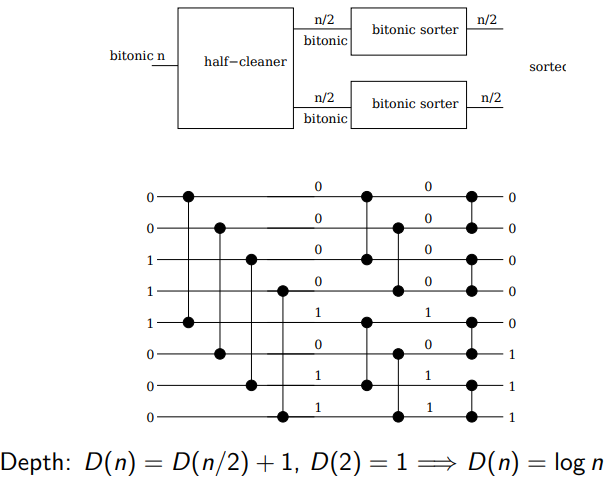
\includegraphics[scale=0.7]{bitonic_sorter}
\end{center}
Using the bitonic sorters on the clean version, while not actually doing anything, keeps the data in the correct place. Supposing the converse where the bottom half was clean with 1s, they would all be in the correct place and concatenating it with the output from the bitonic sorter gives a list
\paragraph{Step 2: A merging network}
Merges 2 sorted sequences. Adapt a half-cleaner.\\
\\
Idea: given 2 sorted sequences, reverse second one, concatenate with the first $\Rightarrow$ bitonic\\
\\
Example:\\
$$X=0011 \quad Y=0111 \quad Y^R=1110 \quad XY^R=00111110$$
\begin{itemize}
	\item So can merge X and Y by doing bitonic sort on X and $Y^R$
	\item Don't explicitly reverse Y, instead reverse the bottom half of the connections of the first half-cleaner
\end{itemize}
\begin{center}
	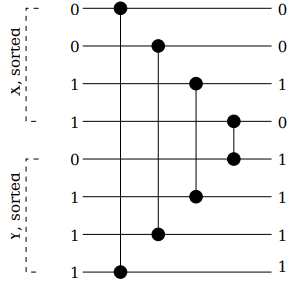
\includegraphics[scale=0.7]{reverse_cleaner}
\end{center}
\begin{center}
	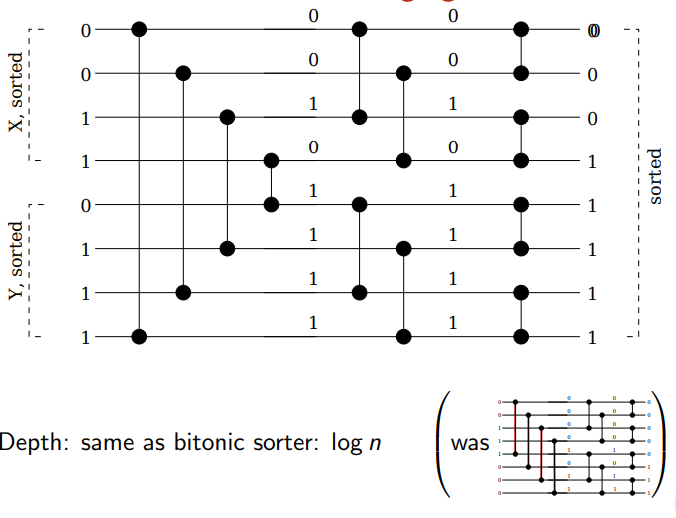
\includegraphics[scale=0.7]{full_network}
\end{center}
\paragraph{Step 3: Asorting network}
Recursive merging - like merge sort, bottom up:
\begin{center}
	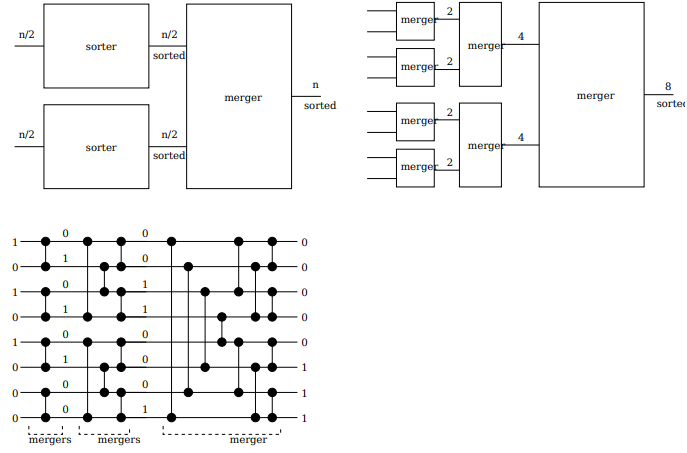
\includegraphics[scale=0.8]{AsortingNetwork}
\end{center}
You can see that this just keeps recursing down the size of the mergers\\
\\
Depth:
$$D(n)=D(n/2)+\log n, D(2)=2 \Rightarrow D(n)=\Theta(\log^2 n)$$
Use 0-1 principle to prove that this sorts all inputs\\
\\
Prove by induction as it has recursive construction.\\
\textbf{Base case}: comparators sort two numbers.\\
Need to prove mergers do what they are supposed to do. - recursive construction so use induction again\\
Need to prove half cleaners do what they are supposed to do - proof already shown via lemma.\\
\section{Shared Memory - NOT EXAMINABLE WOOOOOO}
\subsection{Parallel Random Access Machines (PRAMs)}
Basically, that's what you get when you dream von Neumann's dream in parallel.\\
\\
Bunch of synchronous processors (with little local memory), shared memory; in each step, each processor can access a memory cell in unit time (read or write), or perform local computation
\begin{center}
	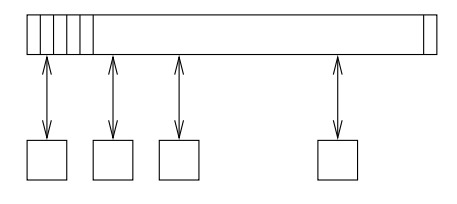
\includegraphics[scale=0.7]{pram}
\end{center}
Various models:
\begin{itemize}
	\item EREW (exclusive read, exclusive write)
	\item CREW (concurrent read, exclusive write)
	\item CRCW (concurrent read, concurrent write)
\end{itemize}
Here: problems with concurrent writes
\begin{itemize}
	\item \textbf{common}: all the same
	\item \textbf{priority}: processors are sorted by priority; if more than one want to write, highest priority wins
	\item \textbf{arbitrary}: arbitrary one wins
	\item \textbf{majority}: many sub models
\end{itemize}
Obviously: $EREW\leqslant CREW \leqslant CRCW$\\
\\
PRAMs in general, and CRCWs in particular, are theoretical models. No real success with building a large one\\
\\
They are, however , extremely nice when one wants to develop parallel algorithms without having to care about, say, network structure\\
\\
The developer can concentrate on algorithmic aspects, rather than messy technical details\\
\\
There are a few ways to (more or less) automatically transform PRAM algorithms into "real" ones\\
\\
Before we can see out first "real" PRAM algorithm, here's the basic extra programming construct
\begin{lstlisting}
for $P_i, 1\leqslant i\leqslant n$ in parallel do
	processor $P_i$ does something
end for	
\end{lstlisting}
\textbf{Example}\\
Suppose we have processors $\seq{P}{1}{n}$, and memory cells, say $A(1),A(2),...$
\begin{lstlisting}
for $P_i, 1\leqslant i\leqslant n$ in parallel do
	A(i)$\leftarrow$ i
end for	
\end{lstlisting}
\subsection{Parallel Mergesort}
Suppose you have an input $S=(\seq{s}{1}{n})$, n power of two (just for presentation)\\
\\
Suppose S pairwise distinct (also no real restriction as can replace $s_i$ by $(s_i,p_i)$ with $p_i$ ID of ith processor)\\
\\
\begin{lstlisting}
Sequence MergeSort (Sequence S)

if |S|$\leqslant 1$ then
	return S
end if
Split S into two sequences $S_1,S_2$ of equal size
$R_1\leftarrow MergeSort(S_1)$
$R_2\leftarrow MergeSort(S_2)$
return Merge($R_1,R_2$)
\end{lstlisting}
As so often, can visualise idea of algorithm using complete binary tree of height $\log n$ (i.e., n leaves)
\begin{itemize}
	\item ith leaf stores ith input element $s_i$
	\item each internal node (non leaf) receives sorted sequence from each of its two children and merges them
	\item this, each internal node v is responsible for sorting the leaves in the sub-tree underneath, i.e., in sub tree with root v
\end{itemize}
\begin{center}
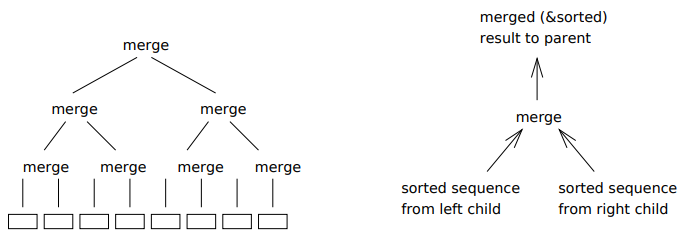
\includegraphics[scale=0.7]{merge}
\end{center}
Let $M(\ell)$ demote time needed to merge two sorted sequences of length $\ell$ each\\
\\
An algorithm that does \textbf{all the mergers on one level in parallel} would then need time
$$\sum _ { i = 0 } ^ { \log ( n ) - 1 } M \left( 2 ^ { i } \right) = O ( M ( n ) \log n )$$
Now, what $M(n)$ can we come up with
\textbf{Definition}
\begin{itemize}
	\item Let $R_1\&R_2$ denote result of MERGE($R_1,R_2$)
	\item \textbf{Rank:} Let S be a sequence and x be an arbitrary element, not necessarily $\in$ S. Then Rank(x,S) is the number of elements from S that are strictly smaller than x
	\item \textbf{Cross rank:} Let S,T be sorted sequences, $S=(\seq{s}{1}{n})$. Let
$$R [ S , T ] : S \rightarrow \mathbb { N } \text { with } R [ S , T ] \left( s _ { i } \right) = \operatorname { Rank } \left( s _ { i } , T \right) , 1 \leq i \leq n$$
We use $R [ S , T ] \text { as vector } \left( \operatorname { Rank } \left( s _ { 1 } , T \right) , \ldots , \operatorname { Rank } \left( s _ { n } , T \right) \right)$
\end{itemize}
Example:
\begin{itemize}
\item S=(1,3,7,9,11), then Rank(8,S)=3 and Rank (3,S)=1
\end{itemize}
\subsubsection{Lemma}
Let S,T be two sorted sequences with $S\cap T=\varnothing$. Then we can compute S\&T on an $\mathcal{O}(|S|+|T|)$-processor CREW-PRAM in time $\mathcal{O}(\log(|S|+|T|))$
\subsubsection{Corollary}
With |S|=|T|=n  we get time $M(n)=\mathcal{O}(\log(n))$
\subsubsection{Proof of lemma}
Let $S=(\seq{s}{1}{n})$. $s_i$ must appear in S\&T at position $Rank(s_i,S\&T)$ . Since $S\cap T=\varnothing$ we have
$$\operatorname { Rank } \left( s _ { i } , S \& T \right) = \operatorname { Rank } \left( s _ { i } , S \right) + \operatorname { Rank } \left( s _ { i } , T \right) = ( i - 1 ) + \operatorname { Rank } \left( s _ { i } , T \right)$$
T is sorted, this can find $Rank(s_i,T)$ in time $\mathcal{O}(\log |T|)$ using binary search. If we've got one processor for each element of S when know $Rank(s_i,S\&T)$ for every $s\in S$ in time $\mathcal{O}(\log |T|)$\\
\\
Do the same for elements $t_i\in T$
\subsubsection{Theorem}
$\mathcal{O}(n)$ -processor CREW-PRAM can sort n number in time $\mathcal{O}((\log n)^2)$ time
\end{document}